%%% LaTeX Template
%%% This template can be used for both articles and reports.
%%%
%%% Copyright: http://www.howtotex.com/
%%% Date: February 2011

%%% Preamble
\documentclass[paper=a4, fontsize=11pt]{scrartcl}	% Article class of KOMA-script with 11pt font and a4 format
\usepackage[margin=0.7in]{geometry}
\usepackage[english]{babel}															% English language/hyphenation
\usepackage[protrusion=true,expansion=true]{microtype}				% Better typography
\usepackage{amsmath,amsfonts,amsthm}										% Math packages
%\usepackage{color,transparent}													% If you use color and/or transparency
\usepackage[hang, small,labelfont=bf,up,textfont=it,up]{caption}	% Custom captions under/above floats
\usepackage{epstopdf}																	% Converts .eps to .pdf
\usepackage{subfig}																		% Subfigures
\usepackage{booktabs}																	% Nicer tables
\usepackage[pdftex]{graphicx}
\usepackage{listings}
\usepackage{lscape}
\usepackage{longtable}
\usepackage{dcolumn}

%%% Advanced verbatim environment
\usepackage{verbatim}
\usepackage{fancyvrb}
\DefineShortVerb{\|}								% delimiter to display inline verbatim text


%%% Custom sectioning (sectsty package)
\usepackage{sectsty}								% Custom sectioning (see below)
\allsectionsfont{%									% Change font of al section commands
	\usefont{OT1}{bch}{b}{n}%					% bch-b-n: CharterBT-Bold font
%	\hspace{15pt}%									% Uncomment for indentation
	}

\sectionfont{%										% Change font of \section command
	\usefont{OT1}{bch}{b}{n}%					% bch-b-n: CharterBT-Bold font
	\sectionrule{0pt}{0pt}{-5pt}{0.8pt}%	% Horizontal rule below section
	}


%%% Custom headers/footers (fancyhdr package)
\usepackage{fancyhdr}
\pagestyle{fancyplain}
\fancyhead{}														% No page header
\fancyfoot[C]{\thepage}										% Pagenumbering at center of footer
\renewcommand{\headrulewidth}{0pt}				% Remove header underlines
\renewcommand{\footrulewidth}{0pt}				% Remove footer underlines
\setlength{\headheight}{13.6pt}

%%% Equation and float numbering
\numberwithin{equation}{section}															% Equationnumbering: section.eq#
\numberwithin{figure}{section}																% Figurenumbering: section.fig#
\numberwithin{table}{section}

\usepackage[parfill]{parskip}
\usepackage{float}
\usepackage{hyperref}
\usepackage[numbers]{natbib}															% Tablenumbering: section.tab#


%%% Title
\title{
	\vspace{-0.5in} 	\usefont{OT1}{bch}{b}{n}
        SEM2220: iOS Word Pairs Assignment \
}

% Authors
\author{
	\usefont{OT1}{bch}{m}{n} Samuel Jackson
	\\ \usefont{OT1}{bch}{m}{n} University Of Aberystwyth
	\\   \texttt{slj11@aber.ac.uk}
}

\date{\today}

\begin{document}

\maketitle

\clearpage

\section{Introduction}
This report provides the documentation for the second assignment of the SEM2220 module. The task of this assignment was to produce a mobile application for the iOS platform. The purpose of the application was to create a language education application that stores and manages ``word pairs'' in both a foreign and native language. The assignment brief specified that users should be able to store various metadata alongside the pairs and can test their knowledge using a revision exercise. This document provides a discussion of how I implemented this application along with evidence of testing and a self evaluation. 

\section{GUI \& Storyboard}
My first step in tackling this assignment was to think about what views would be necessary and how to lay them out in an intuitive way for the user. I began this assignment drawing out a very rough version of the application storyboard on pieces of paper. This made me focus on the type of operations that would need to be performed on the data model. It also helped me to think about how the screens could be organised and the transitions (segues) that would be required. This process also allowed me to think about how to layout each view. I found this to be a slight challenge because I do not own an iOS device and so I am generally less familiar with the various interface components and how they are typically used and laid out. Thinking out these issues on paper allowed me to focus on how to properly present information in a way that is logical for the user.

\begin{figure}[H]
\centering
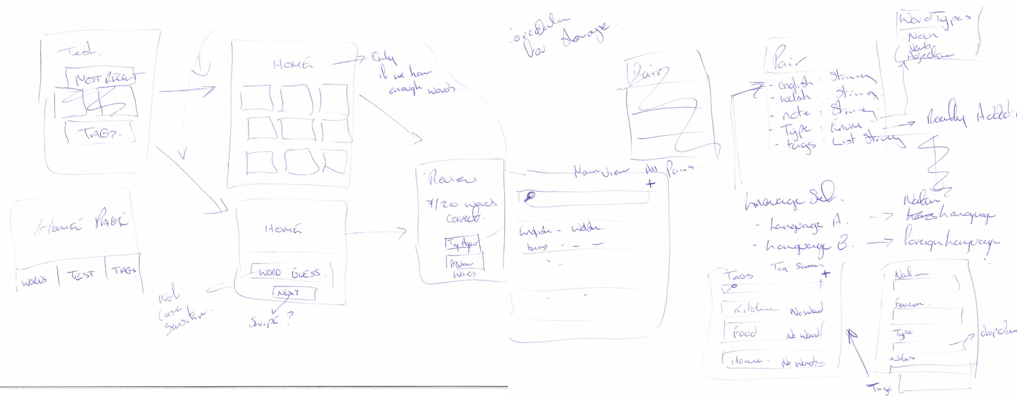
\includegraphics[width=1.0\textwidth]{img/planning.jpg}
\caption{Initial rough planning for the interface \& storyboard. Left: original concepts for the home page and revision exercise. Right: rough plans for the word pairs and tag views.}
\label{fig:planning}
\end{figure}

Based on this initial brainstorming I felt that the application could best be split into three sections. The first section handles the creation and manipulation of word pairs. The second section handles the creation and manipulation of tags which can be associated with word pairs. The third section handles the revision exercise and testing the user. This logical separation of operations is clearly reflected in the user interface. Each of these sections correspond to a different tab on the main tab view when the interface is first opened.

Both the word pairs section and the tags section follow a consistent implementation of CRUD operations. In both cases they are implemented as a table view which lists all of the current items stored in core data. Each of these views uses the plus icon at the top to open a view that lets a user add a new item. Clicking the edit button on the top left of each of these views turns on ``edit mode''. In edit mode items can be removed from the system using the button on the left of the item. Clicking on an item in edit mode will open the item for editing. This recycles the same view that is used for adding word pairs/tags but loads the data for the selected item into the view so that it can be modified by the user.

\begin{figure}[H]
\centering
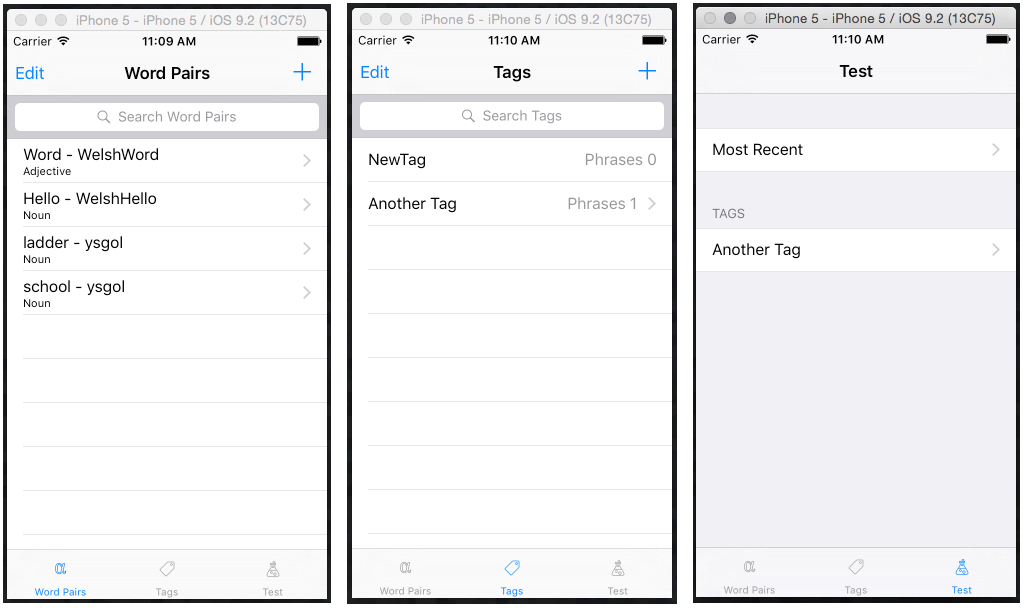
\includegraphics[width=0.8\textwidth]{img/views.jpg}
\caption{The three tab views on the application GUI. Left: The main word pairs view. Middle: The view for managing tags. Right: The test view offering different sets of revision exercises.}
\label{fig:views}
\end{figure}

These two tabs also both implement the additional feature of a search bar. I was initially concerned that this interface was going to become too busy and offer too many operations at this point. However I eventually decided that adding another (separate) view for searching or editing would be lead to too many layers of views to navigate. Encompassing all of this functionality into one view keeps the interface from becoming too deep. The search bar for word pairs allows the user to search either via the foreign \& native word, by type, and by tag. In contrast the search bar for tags can only be searched by name. 

The word pairs section of the application has an additional option on the add button that lets the user choose between creating a new word pair from scratch and importing from a remote URL. This is a very simple interface which allows the user to directly input a URL. If importing from the URL fails for some reason then the user is notified by a message window. The actual loading of the JSON data is performed on a separate thread to avoid interface locking. A loading animation is displayed to the user during this time to inform them that the application is busy. Additionally, if the type of a word is given in lowercase the first letter of the type will be capitalised. This is done using code based on a Stack Overflow question \cite{stringhelper-stackoverflow}.

The third and final section of the GUI is used to test the user via a revision exercise. This provides two different ways to generate an revision exercise. A user can choose to generate a test using the most recent words (based on the time a word pair was added). The second way is to generate a test exercise based on words associated with a particular tag. Tags with no associated words are not shown. Tests are carried out by simply requiring the user to enter the correct word in the other language. At the end of an exercise the user is shown how many they got correct and is given an option to retry the test. 

I found that this part of the application required a little bit of extra work. Swift does not have an array shuffling function by default. I chose to use some code from a public GitHub Gist \cite{arrayshuffle-gist} which would add this feature. Secondly, I found that I required several pieces of data to be passed between the three views. I chose to simplify this by using a class to encapsulate the data as a single object.

Generally speaking I found that one of the most difficult aspects of implementing this project was realising how various segues work, as well as how to send and manage them both automatically and manually. Implementing the project became easier as my understanding how these worked improved. Another issue I found with this project that I would try to tackle better if I were to write this project again is the reuse of views. There are several parts of the application that share similar functionality. Ideally I would have liked to have refactored my code to manage this better. Further developing my understanding of iOS views and Swift in general would help.

\section{Data Model}
In my implementation the core data model sticks very closely to the one provided in the assignment brief. There are two slight modifications that I have made to the original model which I will justify here. The first change modifies the names of the word pairs in the code from ``English'' and ``Welsh'' to ``Native'' and ``Foreign'' respectively. I made this change because I feel it's more extensible. It lends itself to storing alternative languages with the application. It is also potentially more open to modification later to add support for multiple sets of word pairs. 

The second change is the addition of a \textit{timeAdded} member to the \textit{WordPharsePair} entity in the core data model. This is to make it possible to provide a revision exercise based on the most recent word pairs added to the system. This is implemented as an NSDate object. When a new word pair is created by a user then current time is added to the record that is stored in core data. This is never updated even if the user edits the pair at a later date. The case where word pairs are imported from a remote URL is more complex. If JSON data imported from a remote URL includes an element called \textit{timeAdded} and is a string in the NSDate format ``HH:mm'' then this will be used as the value for for the \textit{timeAdded} property in core data. If this element is omitted in the JSON file then the current date and time at the point of local creation will be used instead. 

\begin{figure}[H]
\centering
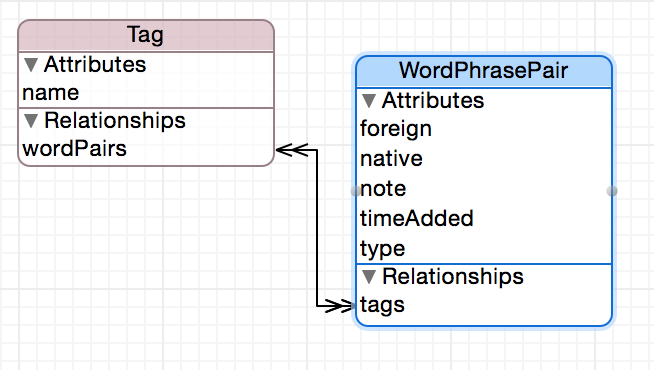
\includegraphics[width=0.6\textwidth]{img/coredata.png}
\caption{The core data model in the final application. Note that slight differences in naming and the additional property in the WordPhrasePair entity.}
\label{fig:core-data}
\end{figure}

I found core data relatively easy to work with. The only real issue that I encountered with this is when the model became out of sync with the code base. I found I had to learn how to migrate the core data model to a new version. Another issue I had with core data is that it has some ``magic'' functions to set properties that represent many to many relationships between tag and word pair entities. As a newcomer to the platform this wasn't entirely obvious and did lead to a loss of development time.

\section{Self Evaluation \& Further Work}
I feel that I have made a good attempt at this project. I have no prior experience with the Swift language or iOS development and I do not even experience using the iOS platform. I feel that I have produced a passible application that fulfils all of the functional requirements of the brief. I feel that I have made a reasonable attempt to conform to the familiar way in which iOS applications work and have not deviated too far from how other applications are laid out. Based on these conclusions I would award myself an A grade with room for improvement.

If I had more time on this project I have several suggestions for what could be improved or developed further. The testing section could be expanded to use several different types of testing. For example the native and foreign word input could be flipped randomly so that the user is given a foreign word and must enter the native equivalent. Another idea would be to use a collection view (or similar) which shows multiple pairs of words that the user must ``tap to match'' similar to the functionality offered in mobile applications such as Duolingo \cite{duolingo}. Another improvement I would like to make would be to add functionality to have multiple collections of word pairs. For example one collection for English and Welsh word pairs and one for English and German word pairs. This would be an easy extension to the core data model and could be implemented as an additional tab on the main interface or a side menu which allows the user to choose the collection to use. 

\clearpage

\begin{landscape}
\section{Test Table}

\begin{longtable}{|l|p{2cm}|p{5cm}|p{5cm}|l|p{5cm}|p{5cm}|}
\hline
\textbf{\#} & \textbf{Functional Requirement} & \textbf{Test Description}                            & \textbf{Expected Outcome}                                                                                                                                                                                                                  & \textbf{Pass/Fail} & \textbf{Actual Outcome}                            & \textbf{Solution}                                                                                                                                                                                                          \\ \hline \hline \endhead
1  & FR1                    & Add new word pair                                    & A new word is added and is shown in the main word pairs view.                                                                                                                                                                              & Fail      & High level exception thrown when setting the data. & The model had recently just been updated through refactoring. Incrementing the version solved this issue.                                                                                                                  \\ \hline
2  & FR1                    & Add new word pair with no type                       & A new word is added without  type and is shown in the main word pairs view.                                                                                                                                                                & Pass      & As Expected                                        & N/a                                                                                                                                                                                                                        \\ \hline
3  & FR1                    & Add new word pair with a note                        & A new word pair is added and a note is shown when clicking on it and viewing it.                                                                                                                                                           & Pass      & As Expected                                        & N/a                                                                                                                                                                                                                        \\ \hline
4  & FR1                    & Edit a word pair and change the content              & Word pair is edited and the details are saved the viewed after editing                                                                                                                                                                     & Pass      & As Expected                                        & N/a                                                                                                                                                                                                                        \\ \hline
5  & FR1                    & Delete a word pair                                   & Deleting a word pair should remove remove it from the table view and remove it from core data. Closing a reopening the app should show the entry is still removed.                                                                         & Pass      & As Expected                                        & N/a                                                                                                                                                                                                                        \\ \hline
6  & FR2                    & Create a new tag                                     & A new tag is created                                                                                                                                                                                                                       & Pass      & As Expected                                        & N/a                                                                                                                                                                                                                        \\ \hline
7  & FR2                    & Assign a tag to an existing word pair                & Viewing the word pair should show that a tag is associated with it                                                                                                                                                                         & Pass      & As Expected                                        & N/a                                                                                                                                                                                                                        \\ \hline
8  & FR2                    & View a list of words for tag                         & Clicking on a tag should show a list of word pairs that are associated with this tag                                                                                                                                                       & Pass      & As Expected                                        & N/a                                                                                                                                                                                                                        \\ \hline
9  & FR2                    & Cannot view words for a tag that has zero references & Clicking on the tag should do nothing. The row should also have the chevron (\textgreater) removed from the interface to indicate this.                                                                                                    & Pass      & As Expected                                        & N/a                                                                                                                                                                                                                        \\ \hline
10 & FR2                    & Editing a tag                                        & Editing a tag should change update tag. The tag should not lose it’s references to word pairs. Word pairs should show as being associated with the edited name of the tag                                                                  & Pass      & As Expected                                        & N/a                                                                                                                                                                                                                        \\ \hline
11 & FR2                    & Delete a tag                                         & Deleting a tag should remove it from the table view. All word pairs that were associated with the tag should no longer have the tag associated with them                                                                                   & Pass      & As Expected                                        & N/a                                                                                                                                                                                                                        \\ \hline
12 & FR2                    & Assign multiple word pairs a tag                     & All of the tags should be shown in the when viewing the word pair                                                                                                                                                                          & Pass      & As Expected                                        & N/a                                                                                                                                                                                                                        \\ \hline
13 & FR2                    & Remove all tags associated with a word pair          & An association with a tag is optional, so the it should be possible to remove all tags associated with a word pair.                                                                                                                        & Fail      & Tags are not removed.                              & The NSSet holding the tags was not being cleared before adding new tags. This meant that the set was only ever updated with new tags, but removing a tag had not effect. This is now resolved by clearing before updating. \\ \hline
14 & FR3                    & Search for a word pair by foreign/native word        & Searching by a word pair should filter all of the pairs that match either the foreign or the native word                                                                                                                                   & Pass      & As Expected                                        & N/a                                                                                                                                                                                                                        \\ \hline
15 & FR3                    & Search for a word pair by tag                        & Searching by tag should return all words that are associated with that particular tag                                                                                                                                                      & Pass      & As Expected                                        & N/a                                                                                                                                                                                                                        \\ \hline
16 & FR3                    & Search for a word pair by type                       & Searching by type should return all words that are associated with that particular type                                                                                                                                                    & Pass      & As Expected                                        & N/a                                                                                                                                                                                                                        \\ \hline
17 & FR3                    & Editing a word pair while a search filter is active  & Editing a word pair while a search filter is active should edit the correct word. When the filter is removed the edited version of the word pair should be present and correct in the table view                                           & Pass      & As Expected                                        & N/a                                                                                                                                                                                                                        \\ \hline
18 & FR3                    & Removing a word pair while a search filter is active & Removing a word pair while a search filter is active should remove the correct word. When the filter is removed the word pair should no longer be present and correct in the table view                                                    & Pass      & As Expected                                        & N/a                                                                                                                                                                                                                        \\ \hline
19 & FR3                    & Searching for a tag by name                          & Searching by name for a tag should return all of the tags which match the filter value                                                                                                                                                     & Pass      & As Expected                                        & N/a                                                                                                                                                                                                                        \\ \hline
20 & FR4                    & Starting a test set with the most recent words       & A new test set should be generated that only consists of the 10 most recent words added to the application. This collection of words should be randomised.                                                                                 & Pass      & As Expected                                        & N/a                                                                                                                                                                                                                        \\ \hline
21 & FR4                    & Starting a test set using a tag                      & All of the word pairs associated with a tag should be added to used in the test and the word pairs should be randomised.                                                                                                                   & Pass      & As Expected                                        & N/a                                                                                                                                                                                                                        \\ \hline
22 & FR4                    & Entering a correct guess for a word                  & Entering a correct guess should show confirmation that it was correct and display the foreign word.                                                                                                                                        & Pass      & As Expected                                        & N/a                                                                                                                                                                                                                        \\ \hline
23 & FR4                    & Entering an incorrect guess for a word               & Entering an incorrect guess should inform the user that they were wrong and display the correct foreign word.                                                                                                                              & Pass      & As Expected                                        & N/a                                                                                                                                                                                                                        \\ \hline
24 & FR4                    & Cancelling a revision exercise                       & At any point during the test the user should be able to click the cross icon to return the the home screen.                                                                                                                                & Pass      & As Expected                                        & N/a                                                                                                                                                                                                                        \\ \hline
25 & FR4                    & Review a revision exercise                           & The total number of correct guesses and the total number of words in the exercise should be displayed. The user should be able to navigate back to the home screen                                                                         & Pass      & As Expected                                        & N/a                                                                                                                                                                                                                        \\ \hline
26 & FR4                    & Retake a revision exercise                           & On the revision page, clicking the “try again” button restart the test. Entries should be randomised again, but the same words should be reused.                                                                                           & Pass      & As Expected                                        & N/a                                                                                                                                                                                                                        \\ \hline
27 & FR5                    & Importing data from a URL                            & New word pairs should be added on the main screen. A loading spinner should be shown while loading. A message should be shown when the operation successfully completes. Dismissing the message should return the user to the home screen. & Pass      & As Expected                                        & N/a                                                                                                                                                                                                                        \\ \hline
28 & FR5                    & Importing data from an invalid URL                   & The operation should fail and a message should be displayed to the user informing them that it was unsuccessful. They should not be segued back to the main screen.                                                                        & Pass      & As Expected                                        & N/a                                                                                                                                                                                                                        \\ \hline
                                                                                                                                                                                                                      
\end{longtable}


\end{landscape}

\clearpage
\bibliographystyle{unsrtnat}
\bibliography{references}
\end{document}
